% !TeX root = ../thuthesis-example.tex

\chapter{绪论}

本章节分析了现有的固定路线定位技术的研究背景和研究意义,介绍了国内外关于视觉惯性定位和地图辅助定位的研究现状,并指出了现有研究的不足之处。本章通过论述核心研究内容,提炼出了文章的创新之处。


\section{课题背景}

近年来,汽车和机器人的智能化是炙手可热的研究和应用方向,而固定路线下运行的智能汽车和机器人是其中的一个重要研究方向。相较于通用智能,在固定路线下应用的智能化技术更容易实现,因此也涌现了一批类似于无人驾驶公交车\cite{stephen2023driverless}、智驾汽车通勤模式\cite{xin2023xinchuxing}、变电站巡检车\cite{song2020xinhuawang}、矿山无人运输机器人\cite{li2023keji}等应用场景,如图~\ref{fig:apply} 所示。

\begin{figure}[htbp]
  \centering
  \begin{subfigure}[b]{0.45\textwidth}
      \centering
      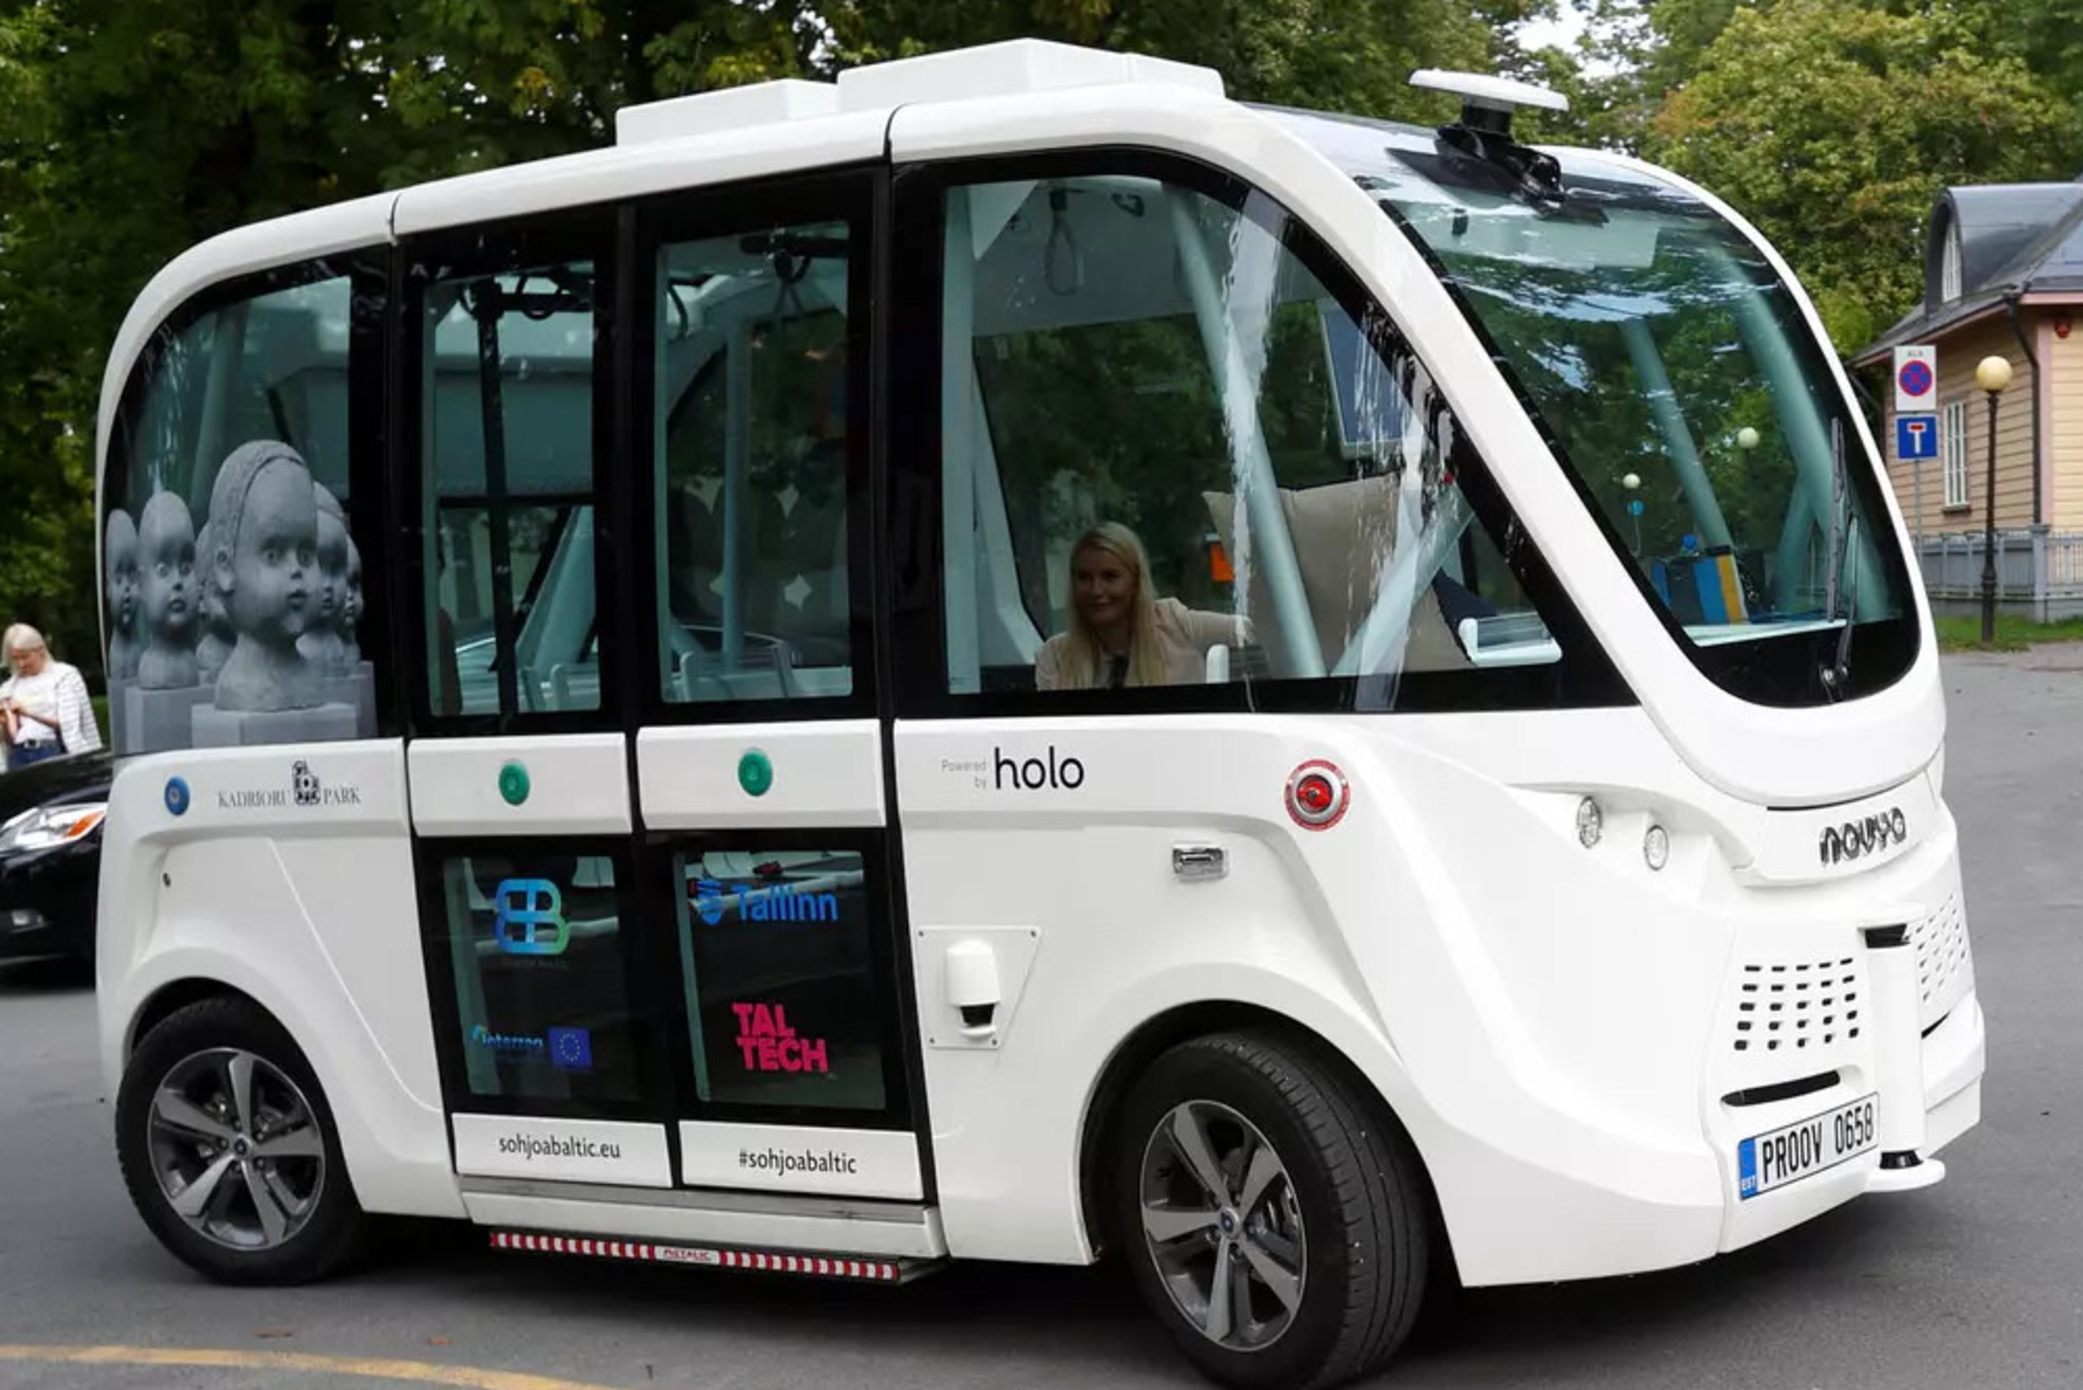
\includegraphics[width=\textwidth]{Apply1.pdf}
      \caption{无人驾驶公交车\cite{stephen2023driverless}}
      \label{fig:apply_sub1}
  \end{subfigure}
  \begin{subfigure}[b]{0.45\textwidth}
      \centering
      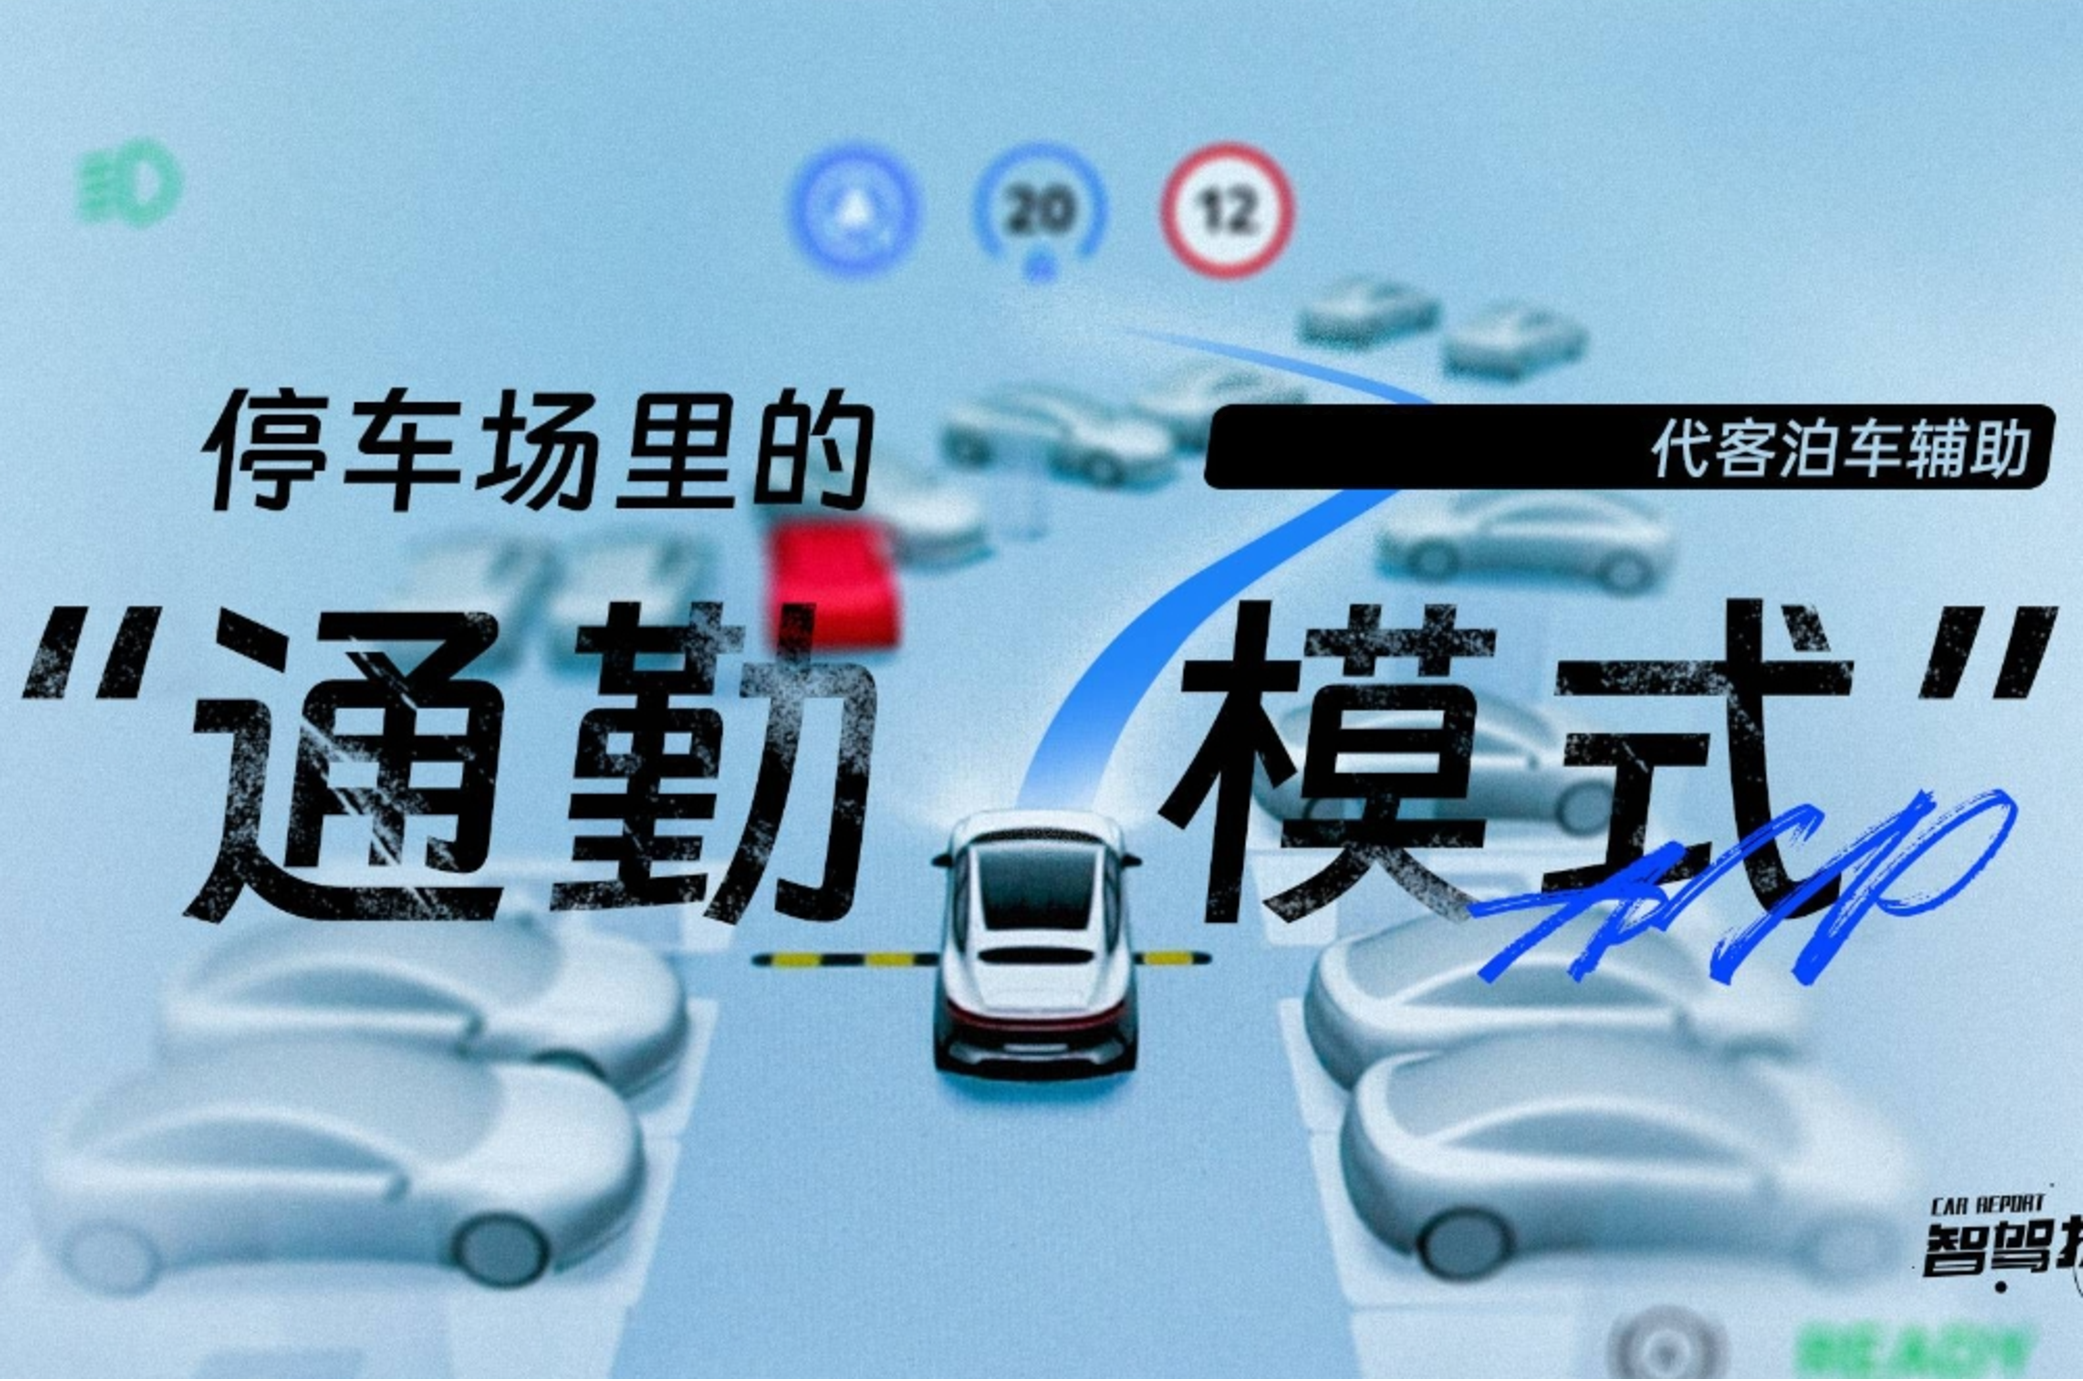
\includegraphics[width=\textwidth]{Apply2.pdf}
      \caption{智驾汽车通勤模式\cite{xin2023xinchuxing}}
      \label{fig:apply_sub2}
  \end{subfigure}
  \begin{subfigure}[b]{0.45\textwidth}
      \centering
      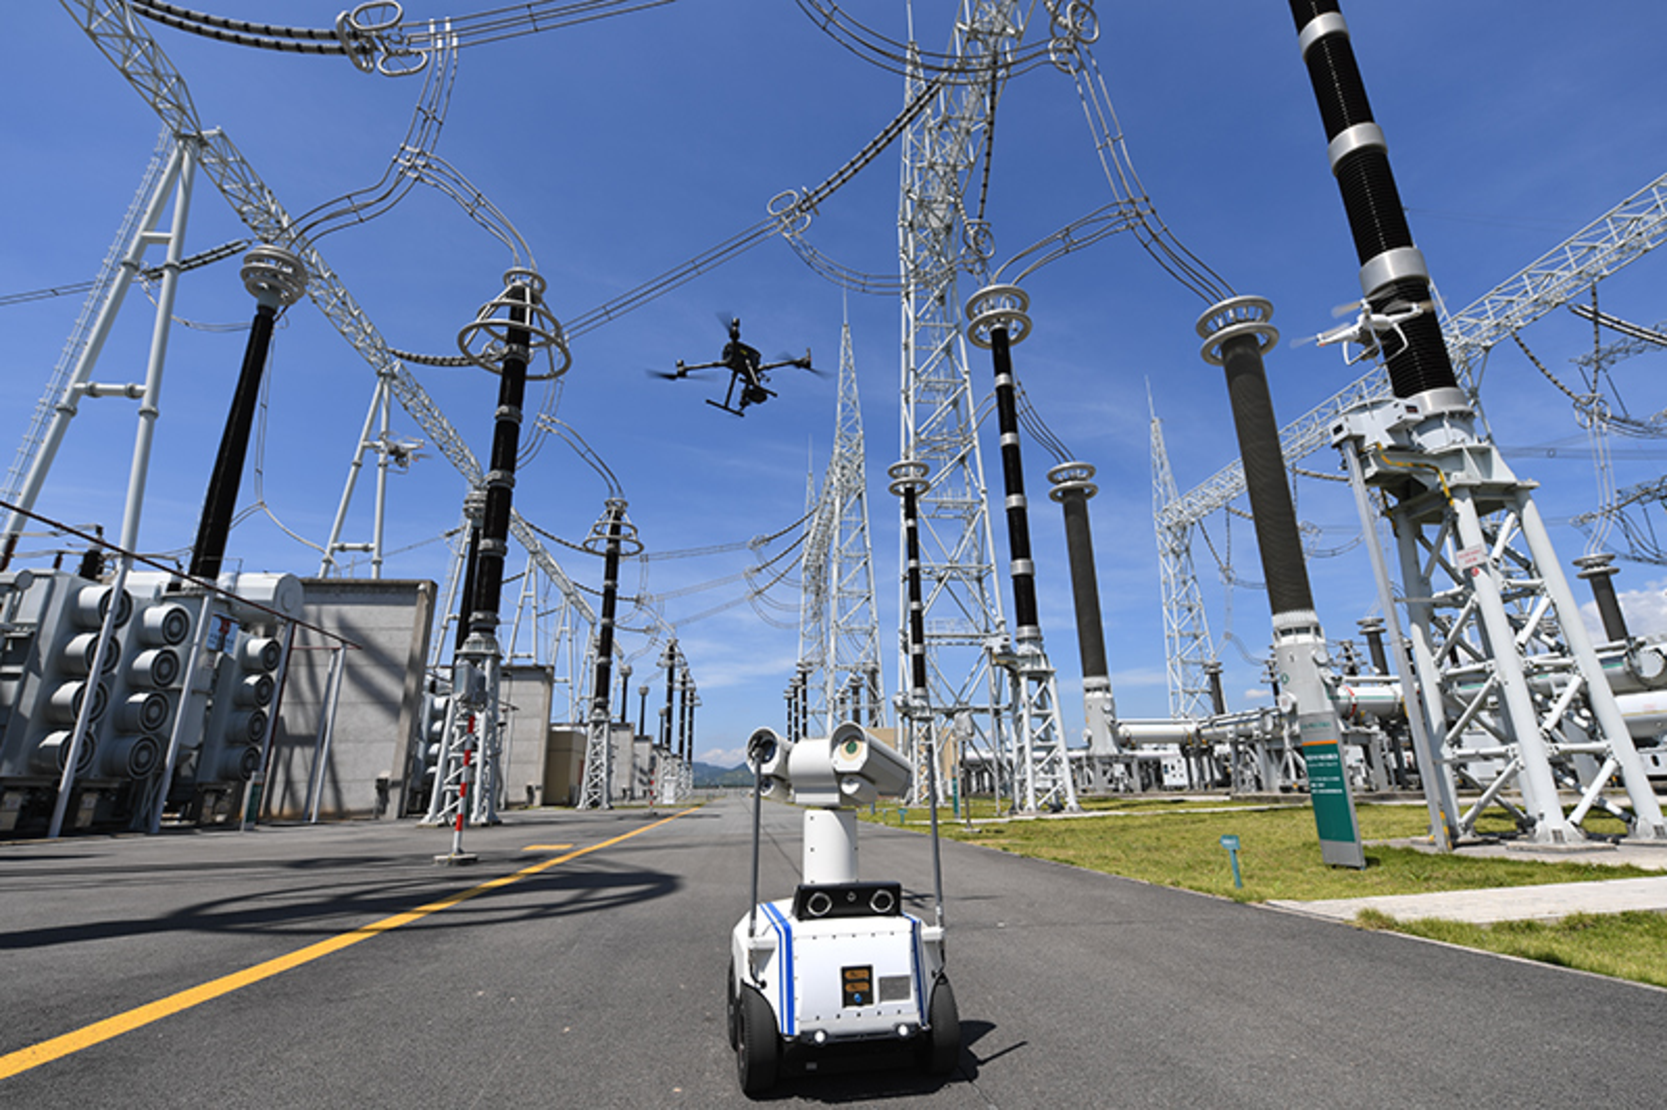
\includegraphics[width=\textwidth]{Apply3.pdf}
      \caption{变电站巡检车\cite{song2020xinhuawang}}
      \label{fig:apply_sub3}
  \end{subfigure}
  \begin{subfigure}[b]{0.45\textwidth}
      \centering
      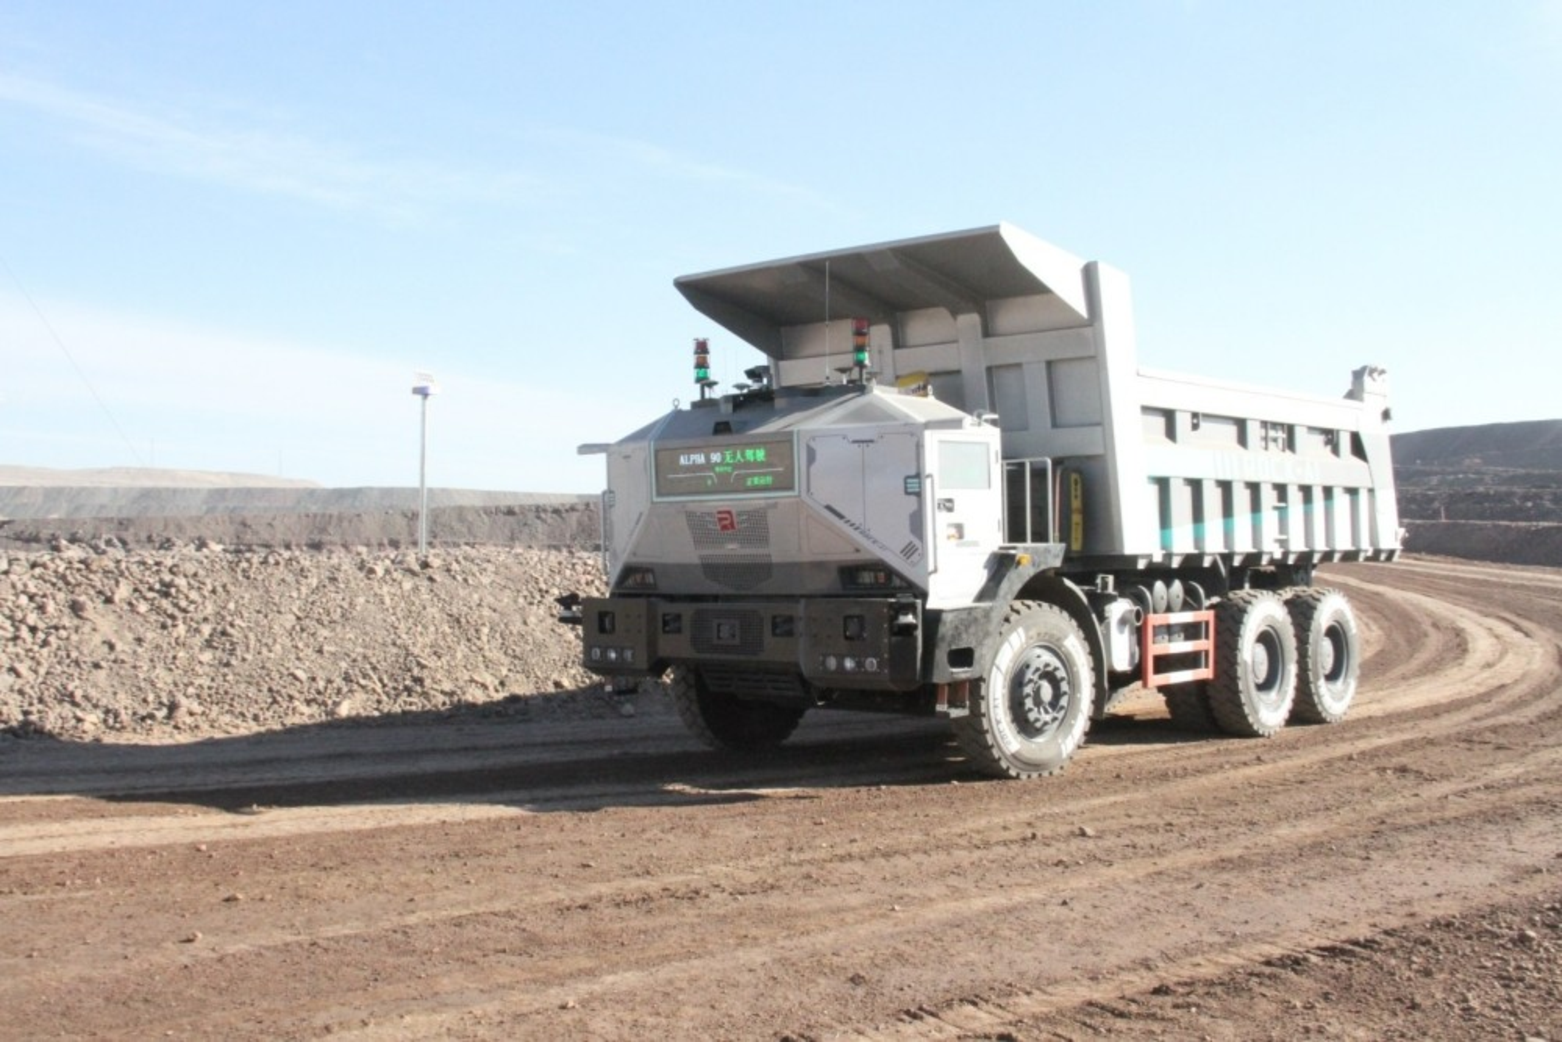
\includegraphics[width=\textwidth]{Apply4.pdf}
      \caption{矿山无人运输机器人\cite{li2023keji}}
      \label{fig:apply_sub4}
  \end{subfigure}

  \caption{固定路线定位的应用场景}
  \label{fig:apply}
\end{figure}

在这些应用中,汽车和机器人运行在提前设置好的固定路线上,通过自身所具备感知能力对环境做出反馈,完成规划、导航等更复杂的任务。而在感知能力中,定位是最基础但是却最关键的感知能力之一,定位系统是智能汽车和机器人运行的最基础系统之一。因此,固定路线中的精确定位是一项具有较高实用价值的基础性研究,只有实现了高精度的定位,才能确保复杂任务的可靠实施,才能保证整个智能体的安全。

在定位方法中,视觉惯性定位(Visual-Inertial Localization)是一种应用广泛的定位形式,它通过融合视觉和惯性传感器的数据,实现对自身位置的估计。视觉传感器可以获取环境的视觉信息,而惯性传感器,例如惯性测量单元(Inertial Measurement Unit, IMU),可以获取自身的运动信息,两者结合可以实现对自身位置的估计。视觉惯性定位方法具有定位精度高、成本低、易于实现等优点,因此在固定路线定位中得到了广泛的应用。然而,视觉惯性定位方法也存在一些问题,例如视觉传感器易受光照、天气等环境因素影响,惯性传感器易受积分漂移等因素影响,这些因素都会影响视觉惯性定位的精度。因此,如何提高视觉惯性定位的精度,是当前固定路线定位研究的一个重要问题。

一种主要的改进方式是通过引入卫星导航系统(Global Navigation Satellite System, GNSS)信息来提高视觉惯性定位的精度。一般的商用低成本单频GNSS的精度在10米左右,这对于需要精确位置的智能化车辆和机器人来说是远远不够的。为了改进单频GNSS的精度,近年来出现了一些高精度的增强GNSS方法,例如精密单点定位(Precise Point Positioning, PPP)\cite{zumberge1997precise}技术和实时动态载波相位差分(Real Time Kinematic, RTK)\cite{fotopoulos2001overview}技术。PPP和RTK可以将GNSS的定位误差缩减至厘米级,是非常理想的高精度定位方法。但是PPP却因为需要较长的初始化时间\cite{bisnath2018innovation},所以不适合应用在实时定位场景上。而RTK虽然有不错的实时性,但是却经常容易受到天气、温度或者遮挡等问题的影响而产生单次误差较大的定位结果\cite{li2022review}。因此,直接引入GNSS观测信息会受到多种限制,并且高精度的GNSS服务也需要额外的费用,这对于一些低成本的固定路线定位系统来说是不可接受的。

\begin{figure}
  \centering
  \subcaptionbox{人类可理解语义地图\label{fig:sd_map}}{\includegraphics[width=0.45\linewidth]{SD_Map.png}}
  \subcaptionbox{视觉点云地图\label{fig:pc_map}}{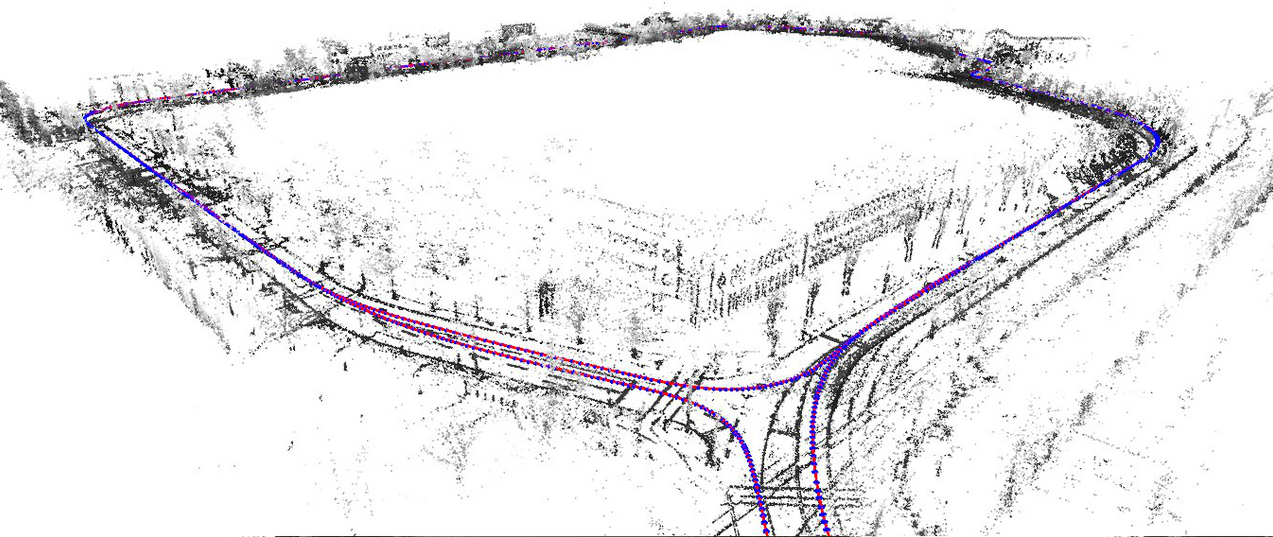
\includegraphics[width=0.45\linewidth]{sparse_pcmap.png}}
  \caption{不同类型的地图}
  \label{fig:maps}
\end{figure}

另一种改进方式是通过引入地图信息来提高视觉惯性定位的精度。此处所指的地图并非是人类理解的语义地图~\ref{fig:sd_map},而是稀疏点云地图,如图~\ref{fig:pc_map}所示。点云地图由图像、拍摄图像的相机位置与姿态,图像特征点及其空间坐标所构成,是一种适合计算机存储和使用的地图。地图信息可以提供给视觉惯性定位系统一个先验的位置信息,从而可以减小定位误差。在固定路线条件下,由于车辆或机器人运行的路线是固定的,因此可以提前获取到路线的地图信息,这方便视觉惯性定位系统使用地图先验信息。除此之外,因为地图信息的收集过程并不受限于天气、温度等环境因素,而且没有实时性要求,可以在精心选择的条件下进行。因此,还可以融合高精度GNSS信息来提高建图精度。地图可以一次建立、多次使用,后续的使用成本相较于高精度GNSS服务要低廉得多。因此,引入地图信息是一种非常理想的提高视觉惯性定位精度的方法。

总的来说,固定路线中的视觉惯性定位是一项有着广泛应用的基础技术,但目前受限于视觉惯性定位技术本身的局限性,其精度还有待提高。在目前可选的改进方法中,引入地图信息是一种非常理想的提高视觉惯性定位精度的方法。因此,本文将围绕固定路线中的视觉惯性定位方法展开研究,通过解决地图构造、地图识别和地图使用等问题来提高定位的精度,提出一种精度满足需求,且具有实际操作性的固定路线中的视觉惯性定位方法。


\section{研究意义}

(1) 以视觉惯性定位为基础,引入地图信息提高定位精度,是当下一种较为新颖的固定路线定位方法,本文将围绕这一方法展开研究,对提高固定路线中的智能汽车和机器人的定位精度具有理论意义。

(2)固定路线中的定位是自动驾驶和机器人领域中一项基础但重要的技术,本文针对这一技术开展研究,对提高固定路线中的智能汽车和机器人的定位精度具有实践意义。

(3)本文在地图的构建和使用中不仅有传统的空间计算、状态估计和非线性优化技术,还引入了基于深度学习的计算机视觉技术,对于推动传统定位技术和深度学习技术的融合具有一定的实践意义。


\section{国内外研究现状}
\subsection{视觉惯性定位}

视觉惯性定位是一种融合了视觉、惯性信息的定位方法,其中视觉信息一般来源于图像、视频等,而惯性信息则一般依靠IMU采集。视觉惯性定位方法以视觉定位和惯性定位技术为基础,但是目前的视觉惯性定位技术一般以视觉定位技术为核心,而惯性定位技术作为补充或约束信息加入到视觉定位中,因此介绍视觉惯性定位的发展有必要从视觉定位技术的发展说起。

% \subsubsection[short]{视觉定位方法}

\begin{figure}
  \centering
  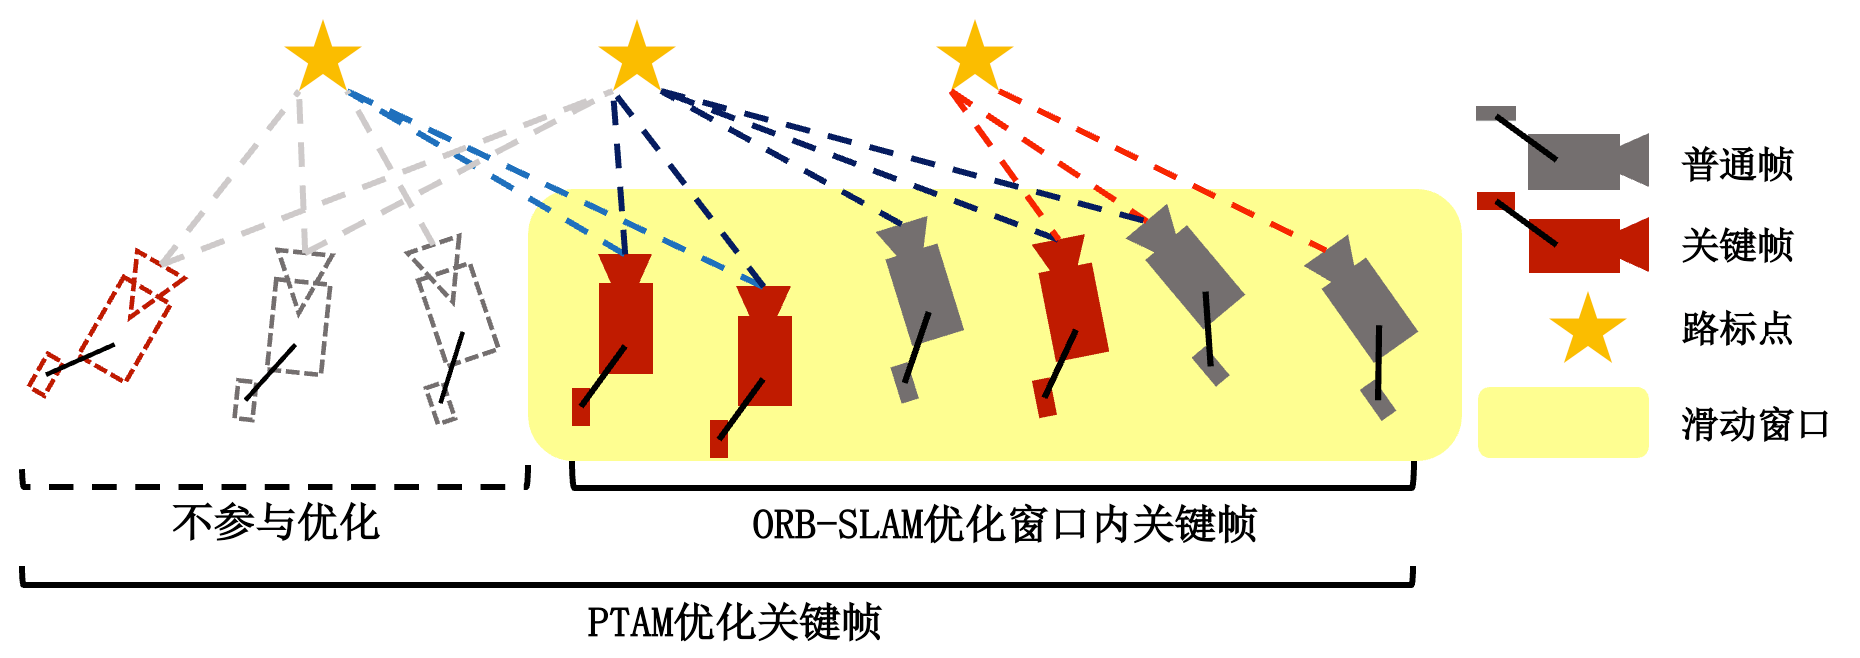
\includegraphics[width=0.9\linewidth]{vo_window.png}
  % \caption*{视觉定位中的关键帧和滑动窗口}
  \caption{视觉定位中的关键帧和滑动窗口}
  \label{fig:vo_window}
\end{figure}

视觉定位中常用的技术之一是同步定位与地图创建(Simultaneous Localization And Mapping, SLAM)。\citet{davison2007monoslam}于2007年首次提出了使用单目图像进行定位的方法MonoSLAM,以扩展卡尔曼滤波器(Extended Kalman Filter,EKF)为核心,实时对图像观测到的特征点进行位置估计,构建3D概率稀疏地图,然后使用地图点对相机位置和姿态进行估计,这是第一种能够达到实时的视觉定位方法,它使得利用视觉信息估计姿态成为可能。同年\citet{klein2007parallel}也提出了一种基于单目图像的定位方法PTAM(Parallel Tracking And Mapping) ,与MonoSLAM不同的是,PTAM的核心估计方法从扩展卡尔曼滤波器改变为光束法平差(Bundle Adjustment, BA)\cite{triggs2000bundle}。BA是一种非线性优化方法,其根据同一个地图点在多个图像上的观测位置,同时优化图像拍摄时相机的位姿和地图点的空间坐标。因为一次优化使用的数据更多,所以这种方法相比于滤波器更准确,但是计算量更大,所以PTAM引入了关键帧的概念:只对关键帧进行光束法平差,而对于普通帧则使用关键帧对其进行约束和定位估计。

PTAM 的另一大进步是将定位与建图两个功能解耦,使两个功能分别同时进行,而这一优点被\citet{mur2015orb,mur2017orb}吸取,创造出ORB-SLAM。ORB-SLAM是一个包含3个主要线程的完整SLAM系统:实时特征点跟踪(Tracking)线程、局部建图优化(Local Mapping)线程、回环检测(Loop Closing)线程。ORB-SLAM中不仅继承了PTAM的关键帧思想,还使用了如图\ref{fig:vo_window}所示的滑动窗口概念,进一步提高了系统实时性。滑动窗口设置包含固定数量关键帧的窗口,随着系统的工作,窗口随时添加新的关键帧并舍弃距离现在最远的关键帧,BA只优化当前窗口内关键帧及其地图点的信息。ORB-SLAM基本奠定了后来视觉定位方法的范式,其提出的3个功能模块也组成后续视觉定位方式的基本骨架。

虽然视觉定位的发展取得了一些进步,但是视觉定位的系统性缺陷却阻碍其应用。在视觉定位研究最广泛的单目视觉定位方面,其依靠的单目相机传感器天然缺少对深度的观测,这造成了单目视觉定位的尺度不确定性,即单目视觉定位不能获得真实世界尺度下的定位结果。为了解决这个问题,研究者们开始在视觉定位的基础上加入了可以获取真实世界尺度信息的传感器,例如惯性测量单元(Inertial measurement unit, IMU),提出了视觉惯性定位。

% \subsubsection{视觉惯性定位方法}
视觉惯性定位是视觉定位和惯性定位的结合,涉及到多传感器信息融合,根据融合方式可以分为松耦合\cite{lynen2013robust}与紧耦合\cite{falquez2016inertial}。松耦合方式是将视觉定位和惯性定位分开处理,让两种定位方式独立运行,然后对结果再进行融合,融合的方式可以选择扩展卡尔曼滤波或者非线性优化。松耦合的优点是系统简单,估计量少,因此不论是运行效率还是灵活度都非常高;缺点是忽略了两种定位方式之间的约束关系,所以精度较差。目前主流的视觉惯性定位基本是紧耦合方式,紧耦合需要将两种定位方式的估计量作为一个整体同时优化。

紧耦合视觉惯性定位方法最早以滤波器的形式发展,此时视觉惯性定位依旧是以IMU运动模型为核心,以线性化和观测性为主要研究方向,最突出的工作是\citet{mourikis2007multi}提出的多状态约束卡尔曼滤波(Multi-State Constraint Kalman Filter,MSCKF),该方法以IMU位置、姿态、速度等状态量和固定数量的相机位置、姿态为主要的估计参数,并没有将地图点加入到优化列表中。MSCKF工作的最主要贡献在于推导出一种测量模型,该模型能够表达从多个相机位姿观察到静态特征时出现的几何约束。

此后,许多基于MSCKF的工作相继提出,框架整体的精度和鲁棒性得到了不断的提升,例如\citet{li2013high}在MSCKF的基础上提出的MSCKF 2.0以及\citet{sun2018robust}提出的双目视觉版本MSCKF。\citet{bloesch2017iterated}提出了一种基于迭代扩展卡尔曼滤波器(Iterated extended Kalman filter,IEKF)的直接法单目视觉惯性里程计ROVIO(RObust Visual Inertial Odometry)。在视觉方面,该方法将地图点在图像中对应点周围的图像块作为路标点的描述子,从而得到光度误差,然后将光度误差进行变换得到IEKF中的启发项,进而进行滤波状态的更新。整体的滤波方程的构造是以IMU为中心进行构造的,保证能观状态不受不断增长的全局协方差的影响,这样可以减小因非线性而造成的误差。

\begin{figure}
  \centering
  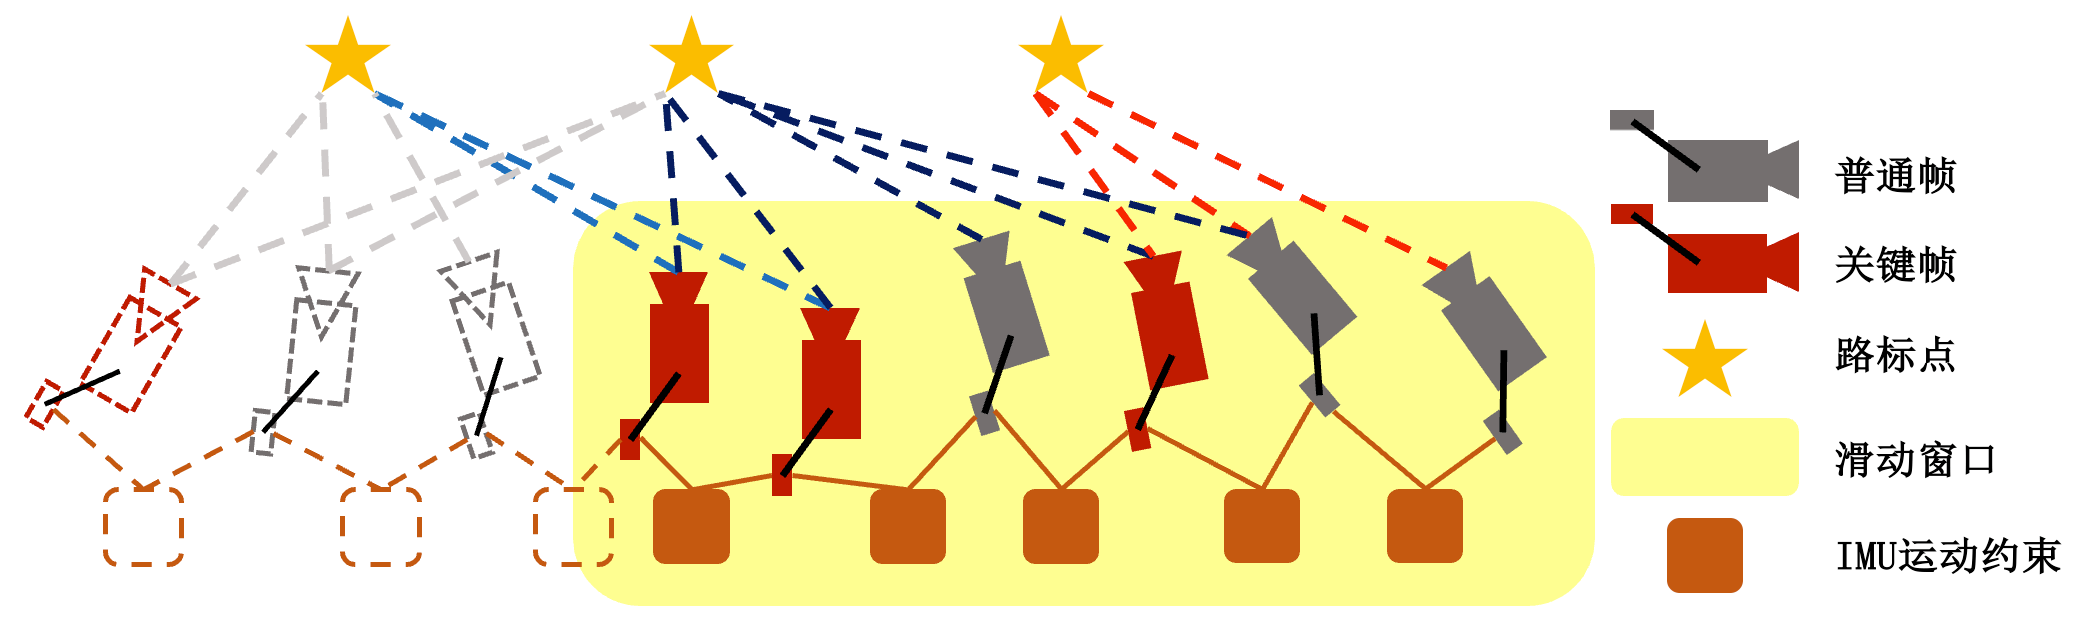
\includegraphics[width=1.0\linewidth]{vio_window.png}
  \caption{视觉惯性定位中的关键帧和滑动窗口}
  \label{fig:vio_window}
\end{figure}

近年来随着非线性优化在视觉定位中的广泛应用,视觉惯性定位方法也尝试使用这种优化方式。参考视觉定位中将地图点和相机位姿以图(Graph)的形式联系起来,然后使用光束法平差进行统一优化,视觉惯性定位在相机位姿之间加入由IMU数据组成的运动约束项,如图\ref{fig:vio_window}所示。IMU运动约束指的是IMU预积分,\citet{forster2016manifold}提出了应用于视觉惯性里程计中的基于四元数的预积分公式,将传统的IMU运动积分公式转化为帧间增量的形式,并且将运动积分中的IMU偏置(Bias)线性化,避免在优化过程中IMU偏置发生变化时重新积分,提高运行效率。\citet{leutenegger2015keyframe}提出的OKVIS(Open Keyframe-based Visual-Inertial SLAM)利用基于关键帧的滑动窗口进行批量非线性优化,先于滑动窗口的关键帧被边缘化,不用来进行估计。系统前端使用多尺度Harris\cite{harris1988combined}特征检测器来提取特征点,然后在其基础上计算BRISK(Binary Robust Invariant Scalable Keypoint)\cite{leutenegger2011brisk}描述子,以便在帧与帧之间进行数据关联。

\citet{qin2018vins}提出的VINS-Mono(Monocular Visual-INertial System)类似于OKVIS,但引入了几个全新的功能,其完整系统包括观测值预处理、初始化、局部视觉惯性联合优化、全局图优化和回环检测5个部分,前端提取Harri特征点,并采用LK光流(Lucas-Kanade opticalflow)\cite{lucas1981iterative}法跟踪相邻帧。VINS-Mono 方法只计算特征点,不计算描述子,同时使用光流法跟踪特征点的运动,这样就减少了计算和匹配描述子的时间和资源。系统采用与 OKVIS 相似的基于滑动窗口的紧耦合位姿估计方法,并且加入了基于词袋模型(Bag of Binary Words,DBoW)\cite{galvez2012bags}的回环检测线程,使系统具有重定位功能。\citet{liu2018ice}提出ICE-BA(Incremental, Consistent and Efficient Bundle Adjustment),沿用VINS-Mono中基于LK光流的特征点跟踪技术,后端则是提出了增量式BA,主要分为3个部分:局部BA、全局BA以及相对边缘化(Relative-Marginalization),前两者采用增量式方法提升了后端速度,后者保证了局部BA和全局BA的一致性。

一些视觉定位方法也发展出了融合惯性信息的版本,\citet{campos2021orb}在ORB-SLAM的基础上提出了ORB-SLAM 3,引入IMU尝试解决在快速运动时丢失特征点的问题:ORB-SLAM 3分别对ORB-SLAM的3个线程作出修改,用以融合IMU信息:在跟踪线程,基于重投影误差和IMU预积分,建立帧与帧之间的约束关系来构造代价函数,从而得到当前帧位姿的最优估计;在局部建图线程,有了新的关键帧之后,将会对前N个关键帧进行优化,当前的关键帧(第N+1帧)将固定不变;在全局回环检测线程,由于IMU提供了尺度信息,因此全局优化将从7个自由度下降到6个自由度,全局位姿优化将忽略IMU信息,因此不再优化速度和偏差,当完成全局位姿优化后,再根据矫正后的位姿对速度进行矫正。

\textbf{总结而言,视觉惯性定位系统的组成部分至今已基本定型,其主要由视觉SLAM系统的功能组件和预积分的惯性测量处理组成。因此,目前的视觉惯性定位方法仍遵循定位与建图同步的工作逻辑,并没有考虑过如何将先验地图运用到定位工作中。本文为了补充这一研究,希望提出一种地图辅助的视觉惯性定位方法,改变以往定位与建图高度同步的范式,这与此前的工作有较明显的差异。}

\subsection{地图辅助的定位方法}
地图辅助定位是一种车辆定位中常用的技术,常用的地图类型有高精(High-Definition,HD)地图、激光雷达点云地图、视觉重建地图等。\citet{jeong2020hdmi}开发了一种高效的HD地图表示方法,并利用粒子滤波器估计车辆的六自由度(6-Degree Of Freedom,DOF)位姿,该方法实现了分米级精度。\citet{xiao2020monocular}和\citet{guo2021coarse}提出了一种基于HD地图的低成本视觉定位方法。这两种方法综合利用了低级地图特征(如点和线特征)以及结构特征(如地图元素的语义和类别),从而能够精确估计车辆的位姿。尽管上述方法在定位方面取得了令人印象深刻的成果,但它们都依赖于成本高昂的高清地图,这些地图的构建需要细致的数据采集和人工标注。

为了降低对高清地图的依赖,研究者们开始探索基于图像和激光雷达扫描的地图构建方法。\citet{stewart2012laps}开发了一种利用单目相机在由搭载激光雷达传感器的测绘车辆预先生成的三维地图中进行定位的方法。该方法通过将激光雷达反射图像与图像强度进行匹配,并选择NMI(Normalized Mutual Information)最高的合成图像来确定相机位姿。\citet{zuo2019visual}采用基于MSCKF的视觉惯性里程计(Visual-Inertial Odometry, VIO)技术,在由激光雷达生成的点云地图中进行定位。具体而言,他们将点云地图作为观测值以更新MSCKF,从而提升其性能。\citet{lin2021autonomous}则将图像引入到先验地图信息中,其方法通过激光雷达估计位姿,同时利用车载图像构建稀疏点云地图。

近年来,随着视觉三维重建技术的进步,涌现了以SLAM和运动恢复结构(Structure from Motion,SfM)\cite{schonberger2016structure}为代表的地图重建方法。通过SLAM和SfM获得的重建地图一般包含地图关键帧的位姿、稀疏点云结构、稀疏点云特征等要素,这些要素可以在定位时快速提供粗略的位置参考,然后选择该位置附近的局部点云地图与当前定位图像进行细匹配和优化定位。具体来说,重建地图的地图关键帧的位姿可以通过特征点匹配、局部地图优化和全局地图优化等手段获得;重建地图的稀疏点云结构一般是通过提取地图关键帧的特征点,并根据地图关键帧的相对位姿三角化获得;重建地图的稀疏点云特征则是由地图关键帧的特征点描述子组成。在定位过程中,首先将待定位图像的特征点与地图的稀疏点云进行匹配,匹配到足够的地图点后可以使用PnP(Perspective-n-Point)算法直接计算待定位图像的位置和姿态。

在具体的重建地图使用方面,VINS-Mono、VINS-Fusion和ORB-SLAM 3等一些SLAM系统都已具有保存和加载先验地图的功能,这些SLAM系统可以提前在指定场景下初始运行、建图,而在此后的运行中依靠初始运行的结果进行定位。\citet{surber2017robust}提出了一种针对无人机的定位系统,旨在利用相机和IMU,在初始飞行中构建参考地图。在后续飞行中,系统通过VIO和图像匹配技术,将当前观测与参考地图进行对比,实现精确的自我定位。\citet{hao2023global}提出了一种两阶段的视觉惯性定位系统:在初始运行的过程中加入了额外的GNSS信息建图,而在后续运行中保持纯净的视觉惯性定位。在此系统中,初始运行阶段的GNSS信息提供了较强的位置约束,因此其所建地图精度得到了提升。这些地图使用方法思考了如何建立先验地图和实时场景中的特征点匹配关系,从而使用先验地图的精确地图点为当前定位提供参考。

然而,上述方法在匹配过程中依旧使用着传统的手工设计特征,这些特征在匹配精度和鲁棒性上仍有提升空间。除此之外,上述方法的重建地图基本都是基于SLAM系统的,这意味着地图的构建和定位是高度耦合的,系统本身的建图误差会传导、积累到定位过程中。虽然有工作\cite{hao2023global}尝试在建图阶段加入额外位置信息,提升建图效果,但其仍使用注重实时性的SLAM系统进行建图,依然会受到SLAM系统误差累积的影响。为了提升特征匹配的精度,同时降低建图误差对定位的影响,一些研究者开始尝试使用基于深度学习的特征搭配精度较高建图技术,例如SfM或者带GNSS增强的SfM\cite{vincentqin2022colmapgps},来提升整体的定位精度。

\citet{sarlin2019coarse}提出了一种“由粗到细”的地图使用方式:其建图过程使用SfM和具有精确位姿的图片进行;其定位方法首先使用基于深度学习的图片级描述子NetVLAD(Vector of Locally Aggregated Descriptors)\cite{arandjelovic2016netvlad}对定位图片进行粗位置查询,此后使用基于深度学习的像素级描述子SuperPoint\cite{detone2018superpoint}对定位图片的特征点进行细致匹配。这种方法在匹配过程中使用了基于深度学习的特征,从而提升了匹配的精度和鲁棒性,同时具有较高的实时性,为后续许多工作提供了一种地图定位范式。\citet{yang2022real}提出了一种基于视觉重建地图的定位方法,其方法在“由粗到细”定位的基础上引入了VIO,利用实际定位中的帧间相对位姿约束提升了定位精度。\citet{lin2023visual}则更是引入了多地图概念,其方法在匹配过程中使用了多个地图,从而提升了匹配的鲁棒性。近年来,由于深度学习端到端技术的启发,也出现了一些使用隐式地图使用的定位方法,\citet{xue2020learning}提出的GNNMapNet与\citet{wang2023robustloc}所提出的RobustLoc都是这类方法的代表。这类方法使用带有坐标和姿态的图像作为训练集进行训练,在推理时可以只输入图像就端到端地输出定位结果。

\begin{figure}
  \centering
  \subcaptionbox*{GNNMapNet\cite{xue2020learning}定位(红色)效果\label{fig:gnnmapnet}}{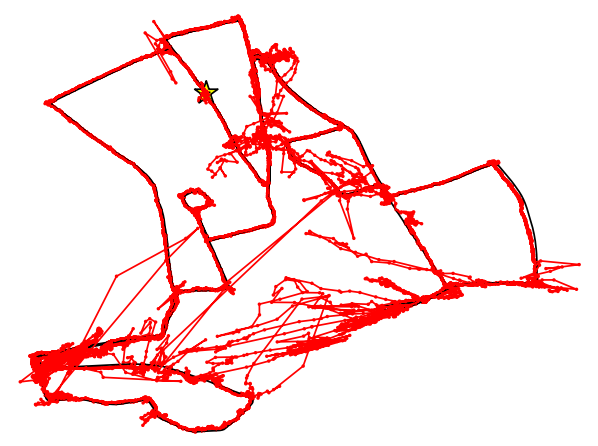
\includegraphics[width=0.45\linewidth]{gnnmapnet.png}}
  \subcaptionbox*{RobustLoc\cite{wang2023robustloc}定位(红色)效果\label{fig:robustloc}}{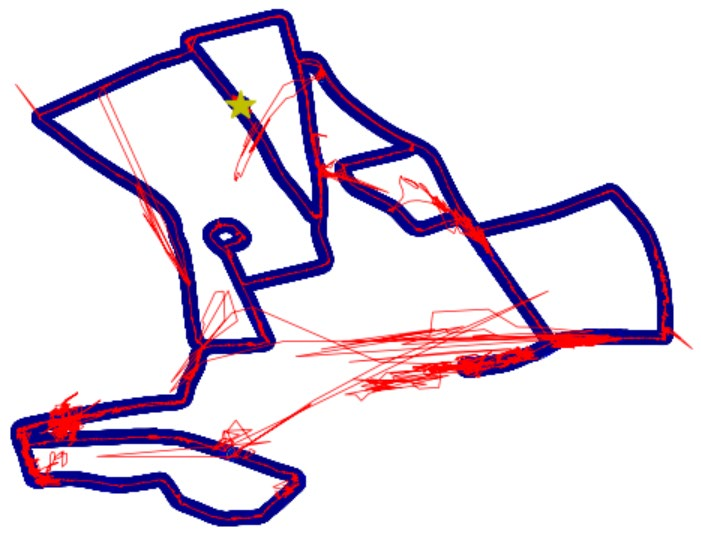
\includegraphics[width=0.45\linewidth]{RobustLoc.png}}
  \caption{端到端定位效果}
  \label{fig:e2eloc}
\end{figure}

虽然这些方法在最终的定位精度上有所提升,但是存在一些问题。首先,这些研究在建图时直接假设地图图片的准确位姿是可获得的,这在实际操作中并不一定总是成立的。其次,这些研究聚焦于先验地图和实际定位之间的匹配关系,并尝试通过各种手段来增加匹配的约束,例如相对位姿、多地图验证等,但是却并没有考虑当地图和定位场景之间产生误匹配时如何降低误匹配的影响。这无疑导致了这些定位方法的脆弱性,使得他们在实际应用中表现出不稳定的性能。此外,\citet{yang2022real}在定位中引入了服务器组件,因此对通信环境的要求较高;\citet{lin2023visual}的方法使用多地图以及丰富的约束,导致运行过程内存占用极大(测试中使用4T RAM);GNNMapNet和RobustLoc这类端到端的定位方法表现极不稳定,产生的轨迹平滑性不足,如图~\ref{fig:e2eloc} 所示。这些问题都限制了上述方法在实际应用中的推广。

\textbf{总结而言,地图辅助的定位方法研究较为分散,根据地图类型的不同,定位方法差异较大。使用HD地图和激光雷达点云地图的方法有较高精度,但是高昂的地图成本却也阻碍着这类技术在实际生产中的应用。基于重建地图的定位方式有较低的成本,但是当前的研究方法中还有一些限制,例如建图假设过强、定位容错不足和实际应用限制较多等问题。为了提供一种实施难度低、容错能力强、完全部署在汽车或机器人上的高精度定位方法,本文希望从建图方式开始,构建完整的固定路线中的视觉惯性定位系统,实现完全部署于车载或机器人端,并具有较高定位精度。}


\section{研究内容与创新}

本文的研究内容是提出一种完整固定路线视觉惯性定位方法,具体而言,本文将通过三个阶段的研究来逐步达成最终目标:(1)先验地图构建;(2)视觉与惯性信息的融合;(3)基于先验地图的位姿优化。


\textbf{(1)先验地图构建:}
辅助地图的构建是本文首先要解决的问题,是剩余其他研究内容的基础。因为SLAM类建图算法由于只进行局部优化,存在误差累积,精度较差的问题,所以本文采用SfM作为基础建图方法,其全局优化策略可以有效降低累计误差。虽然SfM建图具有理论精度高的优势,但原始的SfM建图不具备现实尺度。为了恢复出具有现实世界尺度的地图,必须增加有现实尺度的观测信息,本文所采用的观测信息为高精度GNSS,例如RTK信息。虽然RTK在使用时可能会存在瞬时测量受环境因素影响而产生波动等问题,但是对于建图环节来说,环境可以静心挑选,因此RTK完全可以运用在实际建图中,并且其较高精度的定位观测可以为建图优化提供较好的约束。

本文将着力于融合GNSS观测信息与SfM,提出一种精度较高且稳定性突出的视觉先验地图构建方式。所构建的地图将具有现实世界尺度,且地图关键帧具有较高的位姿估计精度。

\textbf{(2)视觉与惯性信息的融合:}
视觉信息和惯性信息的融合是定位的核心,决定着最终定位的精度如何。目前视觉惯性信息的融合方式主要分为卡尔曼滤波器和非线性优化两种,其中卡尔曼滤波器的优势是在估计矩阵维度较低时计算简单,速度较快,劣势是精度欠缺;非线性优化的方法能够提供较高的精度,且随着硬件技术进步,实时运行非线性优化方法也是可能的。

本文选择以非线性优化作为融合方案,着力于解决如何在非线性优化中构建视觉信息和惯性信息的约束关系,并加入符合固定路线运行的车辆和机器人的合理约束,提高融合后定位精度。

\textbf{(3)基于先验地图的位姿优化:}
在基于地图的定位方法中,建模先验地图在实际定位中的视觉观测,是将地图与定位结合起来的关键。先验地图的视觉观测首先要解决的问题是将地图点与待定位图像特征点进行关联,构建图像特征点观测与图像位置、姿态参数之间的转换关系。基于特征点和描述子的关联方式具有一定的可行性,但是考虑到建图过程可能与实际定位过程有较大的场景表现差异,需要选择对场景差异不敏感的特征点及描述子。除了选择特征点与描述子,基于先验地图稀疏点云的位姿优化也直接关系到定位的精度。先验建图过程中产生的稀疏点云结构,其自身所在的坐标系可能与实际定位时的坐标系并不一致,如何对其坐标系对齐,以及对齐后如何使用先验点云结构来优化实际定位的位姿,是需要解决的问题。

本文将着力于使用一种基于数据驱动的,能够对场景差异较为鲁棒的先验地图视觉观测技术,构建定位与先验建图的关联。在这一基础上提出一种能够对齐先验地图坐标系和实际定位坐标系,以及一种先验地图的合理使用方式来融合先验信息和当下观测,以获得高精度定位结果。

本文的创新点主要体现在以下几个方面:

(1)提出了一种新颖且完整的固定路线视觉惯性定位方法,该方法将先验地图构建、视觉与惯性信息融合、基于先验地图的位姿优化三个阶段有机结合,形成一个完整的视觉惯性定位系统。

(2)在先验地图构建阶段,本文将采用SfM和高精度GNSS观测数据相结合的方式,构建具有现实世界尺度的多层次先验地图,提高地图的精度和稳定性。

(3)在视觉与惯性信息融合阶段,本文提出了一种基于车身运动学约束的视觉惯性里程计,该视觉里程计使用深度神经网络对车身状态进行检测,针对直行状态下的车辆或轮式机器人进行速度观测约束,提高了里程计的估计精度。

(4)在基于先验地图的位姿优化阶段,本文将提出一种新的基于先验地图的位姿优化方法,该方法使用基于深度学习的粗到细定位等手段获得基于先验地图的视觉观测,同时将先验地图的点云结构建模为高斯概率地图,以最大后验概率估计的方式完成位姿优化。

\section{论文组织结构}
本文共六章,各章内容安排如下:

第一章为绪论,首先介绍了本文的研究背景、研究意义,此后根据对国内外研究的调研介绍相关研究进展,通过与现有研究的对比引出本文研究的侧重点,并概括本文的研究内容,最后对全文结构进行介绍。

第二章为系统介绍,首先对整个系统的框架进行了展示,对其中3个主要模块,即离线建图模块、视觉惯性里程计模块和紧耦合地图定位模块进行了详细介绍,分别明确了他们的输出输出已经信息交互关系;此后介绍了该系统中所设计的所有坐标系,为后文统一描述各个模块的内部组成提供了基础;在这之后介绍了离线建图模块的基本过程,包括建图预处理、SfM、建图对齐和建图融合等过程,对每个过程的内部原理做出详细解释;最终介绍了建图模块的输出,即粗细两个粒度的层次先验地图。

第三章为视觉惯性里程计模块介绍,首先从车身运动的情况分类入手,介绍了本文中对于车身状态的三种假设,即静止、直行和转弯;此后介绍了一种以深度学习为基础的车身状态检测方法,该方法使用Transformer网络对惯性信息序列进行分类,以检测车辆处于何种状态;在这之后介绍了一种车身坐标系和IMU体坐标系之间的转换方法,其可以粗略估计两个坐标系的关系;最后介绍了如何将车身状态假设融合到视觉惯性里程计后端优化中,给出了基于车身状态的速度观测约束并求解相关的雅可比矩阵,使得位姿估计问题可以被非线性优化求解。

第四章为紧耦合地图定位模块介绍,首先介绍了基于深度学习的描述子在视觉观测中的优势,由此介绍基于深度学习的粗到细定位方法;此后介绍了转换矩阵初始化和有效性验证,这两部分共同工作,能够完成从视觉惯性里程计定位和粗到细定位的统一,使得多源的定位观测未来可以在统一坐标系下使用;在这之后是紧耦合优化介绍,这一部分详细推导了如何将先验地图建模为高斯概率地图,以及如何以非线性优化的形式完成最大后验概率估计;最后介绍了转换矩阵的更新,论述了其必要性以及详细的转化方法。

第五章为实验与结果分析,首先对实验实施的环境、参数和数据集等信息进行了介绍;此后分别针对本文提出的3个模块进行实验,再对整个系统的性能进行了综合评估,并对实验结果进行了详细的分析,分别从定位精度、定位鲁棒性、定位实时性等方面进行了评估;最后进行了消融实验,更加细致得验证了本文提出的方法的有效性。

第六章为总结与展望,首先总结了本文的研究工作,然后对本文的研究工作进行了展望,提出了未来的改进方向。